%=======================================================================
%  CS-3810 Design Practices in Computer Science -- Assignment 3
%  Project 3: Interactive Data Structure and Algorithms Visualizer
%  Team PY -- Papaa Dennis Morindat, Yididiya Megenta
%
%  Testing, UX and development-plan document. Sections 3-9 answer the
%  Assignment 3 brief directly. Design decisions made by the team are marked
%  [A]; requirements stated or directly implied by the project description
%  are marked [R]. The implementation is submitted separately through the
%  GitHub Classroom repository; this is the design and analysis document.
%
%  Compile with:  tectonic -X compile A3_PY.tex
%  Submission:    rename the compiled PDF to  A3_PY.pdf
%=======================================================================
\documentclass[11pt,a4paper]{article}

\usepackage[T1]{fontenc}
\usepackage{lmodern}
\usepackage[margin=2.05cm,top=2.4cm,bottom=2.4cm,headheight=14pt]{geometry}
\usepackage{amsmath,amssymb}
\usepackage{booktabs}
\usepackage{longtable}
\usepackage{array}
\usepackage{enumitem}
\usepackage{xcolor}
\usepackage{tikz}
\usetikzlibrary{arrows.meta,positioning,fit,backgrounds,calc,shapes.geometric}
\usepackage{listings}
\usepackage{caption}
\usepackage{float}          % [H]: pin floats exactly where they are written
\usepackage{fancyhdr}
\usepackage{microtype}
\usepackage{parskip}
\usepackage{titlesec}
\titlespacing*{\section}{0pt}{2.1ex plus .3ex minus .2ex}{1.0ex}
\titlespacing*{\subsection}{0pt}{1.7ex plus .2ex minus .2ex}{0.7ex}
\titlespacing*{\subsubsection}{0pt}{1.4ex plus .2ex minus .2ex}{0.5ex}
\usepackage[hidelinks]{hyperref}

\setcounter{secnumdepth}{3}
\setcounter{tocdepth}{2}
\setlength{\emergencystretch}{2em}
\setlength{\parskip}{0.35\baselineskip plus 2pt minus 1pt}
\setlength{\textfloatsep}{10pt plus 2pt minus 2pt}
\setlength{\floatsep}{10pt plus 2pt minus 2pt}
\setlength{\intextsep}{10pt plus 2pt minus 2pt} 

\usepackage{tabularx}

%------------------------- colours -------------------------
\definecolor{reqc}{RGB}{0,102,51}
\definecolor{asmc}{RGB}{176,88,0}
\definecolor{primary}{RGB}{11,79,158}
\definecolor{okc}{RGB}{22,120,60}
\definecolor{warnc}{RGB}{176,88,0}
\definecolor{boxc}{RGB}{235,242,250}
\definecolor{statec}{RGB}{232,240,254}
\definecolor{rulec}{RGB}{120,120,120}
\definecolor{codec}{RGB}{245,245,247}

%------------------------- column types -------------------------
\newcolumntype{L}[1]{>{\raggedright\arraybackslash}p{#1}}
\newcolumntype{C}[1]{>{\centering\arraybackslash}p{#1}}

%------------------------- shorthands -------------------------
\newcommand{\R}{\textcolor{reqc}{\textbf{[R]}}}     % stated requirement
\newcommand{\A}{\textcolor{asmc}{\textbf{[A]}}}     % team assumption / decision
\newcommand{\ct}[1]{\texttt{#1}}
\newcommand{\bigO}[1]{\ensuremath{\mathcal{O}(#1)}}
\newcommand{\norm}[1]{\ensuremath{\lvert #1 \rvert}}
\newcommand{\done}{\textcolor{okc}{$\boxtimes$}}
\newcommand{\todo}{\textcolor{rulec}{$\square$}}

%------------------------- code listings -------------------------
\lstdefinestyle{base}{
  basicstyle=\ttfamily\footnotesize,
  columns=fullflexible,
  keepspaces=true,
  breaklines=true,
  breakatwhitespace=false,
  showstringspaces=false,
  frame=single,
  framesep=5pt,
  rulecolor=\color{rulec},
  backgroundcolor=\color{codec},
  xleftmargin=8pt,
  xrightmargin=4pt,
  aboveskip=8pt,
  belowskip=8pt
}
\lstset{style=base}
\lstset{floatplacement=H}
\lstdefinestyle{pseudo}{style=base,numbers=left,numberstyle=\tiny\color{rulec},numbersep=6pt}
\lstdefinestyle{ts}{style=base,numbers=none}
\lstdefinestyle{c}{style=base,numbers=left,numberstyle=\tiny\color{rulec},numbersep=6pt,
  language=C,keywordstyle=\color{primary}\bfseries,
  commentstyle=\color{rulec}\itshape,stringstyle=\color{asmc}}
\lstdefinestyle{sh}{style=base,numbers=none}

\captionsetup{font=small,labelfont=bf,skip=4pt}
\renewcommand{\arraystretch}{1.06}

%------------------------- tikz styles -------------------------
\tikzset{
  comp/.style={draw=rulec, rounded corners=2pt, fill=boxc, align=center,
               inner sep=5pt, font=\small, text width=3.6cm, minimum height=1.35cm},
  layer/.style={draw=rulec, rounded corners=2pt, fill=boxc, align=left,
                inner sep=6pt, font=\small, text width=14.2cm},
  auxbox/.style={draw=rulec, rounded corners=2pt, fill=statec, align=center,
                 inner sep=4pt, font=\footnotesize},
  wf/.style={draw=rulec, fill=white, align=center, inner sep=2pt, font=\scriptsize},
  wfh/.style={draw=rulec, fill=statec, align=center, inner sep=2pt,
              font=\scriptsize\bfseries},
  n/.style={circle, draw=rulec, fill=white, inner sep=1pt, minimum size=4.6mm,
            font=\scriptsize},
  nactive/.style={circle, draw=primary, very thick, fill=statec, inner sep=1pt,
                  minimum size=4.6mm, font=\scriptsize},
  e/.style={-{Stealth[length=2.2mm]}, draw=rulec, thick},
  ed/.style={-{Stealth[length=2.2mm]}, draw=rulec!70, dashed},
  ebi/.style={{Stealth[length=2.2mm]}-{Stealth[length=2.2mm]}, draw=rulec},
  lbl/.style={font=\scriptsize, inner sep=1.6pt, fill=white}
}

%------------------------- headers -------------------------
\pagestyle{fancy}
\fancyhf{}
\fancyhead[L]{\footnotesize CS-3810: Design Practices in Computer Science}
\fancyhead[R]{\footnotesize Assignment 3: Testing, UX, and Development Plan}
\fancyfoot[C]{\footnotesize\thepage}
\renewcommand{\headrulewidth}{0.3pt}

\begin{document}

%=======================================================================
\begin{center}
  {\large\bfseries Department of Computer Science}\\[2pt]
  {\small Ashoka University}\\[10pt]
  {\LARGE\bfseries CS-3810: Design Practices in Computer Science}\\[6pt]
  {\large\bfseries Assignment 3: Testing, UX, and Development Plan}\\[10pt]
  {\large\bfseries Project 3: Interactive Data Structure and Algorithms Visualizer}
\end{center}

%=======================================================================
\section{Project Identification}

\begin{center}
\renewcommand{\arraystretch}{1.25}
\begin{tabular}{@{}L{4.2cm}L{10.4cm}@{}}
\toprule
\textbf{Team Name} & PY. \\
\textbf{Team Members} & Papaa Dennis Morindat, Yididiya Megenta \\
\textbf{Roll Numbers} & 1020241748, 1020241852 \\
\textbf{Assigned Project} & Project 3: Interactive Data Structure and Algorithms Visualizer \\
\textbf{Repository Link} & \url{https://github.com/Ashoka-CS-3810-Design-Practices-in-CS/project-3-PY} \\
\bottomrule
\end{tabular}
\end{center}

\subsection{Assigned Project}

\noindent\textbf{Project title.} Interactive Data Structure and Algorithms Visualizer.

\medskip
\noindent\textbf{Problem statement:} Understanding data structures and algorithms requires more than knowing their steps or final outputs; students must also understand how data changes during execution. However, traditional teaching methods, such as pseudocode and whiteboard demonstrations, often make it difficult to visualize intermediate processes, including pointer movements, node traversal, and comparisons. 

\medskip
\noindent\textbf{Motivation:} This project is driven by the opportunity to make algorithmic learning more interactive and exploratory. By allowing learners to experiment with inputs, control execution, and compare different scenarios, the visualizer aims to encourage curiosity and independent problem-solving. It also provides a way for students to investigate how input characteristics influence algorithm performance, turning abstract concepts into practical learning experiences.
\medskip

\noindent\textbf{Intended users.} \R\ Primary: undergraduate students meeting the
pseudocode for the first time. Secondary: instructors and teaching assistants demonstrating
live, including worst cases. Tertiary: self-learners and interview candidates revising.

\medskip
\noindent\textbf{Main goal of the application.} \R\ The application is aimed at providing an interactive, step-controlled visualizer that allows users to select a data structure and operation, supply or load a dataset, and observe the algorithm's execution one step at a time. The application synchronizes the visual representation of the data structure, the currently executing algorithm line, and auxiliary states such as arrays, stacks, queues, heaps, visited sets, and call stacks. Each step is accompanied by a plain-English explanation and the operation's theoretical time and space complexity, helping learners understand how algorithms work and how their performance is affected by different inputs.

%=======================================================================
\section{Purpose of the Assignment}

\R\ This is the third design-stage deliverable. It translates the Assignment~2 design into an
executable plan for correctness and testing (\S3), complexity and performance (\S4), user
interaction (\S5), risk (\S6), development and integration (\S7) and delivery (\S8), and it
closes with the design-review answers (\S9).

The plan leans on one property of that design: an operation is a pure function that emits a
serialisable, deterministic \ct{Step[]}. The core is therefore tested in Node with no browser,
a committed JSON fixture is a regression oracle, and a UI test is a comparison of two renders
rather than a simulation of an animation. \A\ Where a target cannot yet be met by the current
vertical slice, the section says so and names the phase in \S7 that owns it.

%=======================================================================
\section{Correctness and Testing Plan}

Testing will be carried out throughout development, rather than only before the system launch. Individual components will be tested as they are built, followed by integration testing as they are connected. Before launch, we will test the complete system to identify any remaining issues. We will also rerun relevant tests whenever changes are made to catch potential bugs. The testing plan includes unit, integration, boundary-case, invalid-input, UI interaction, and performance testing to verify the correctness and reliability of the data structure visualizer.

\subsection{Unit testing}

Unit testing will focus on testing individual components, such as data structures, algorithms, input validators, trace generators, and playback controllers, separately. These tests will run in Node without requiring the user interface or a browser, making them faster and easier to run.

For each algorithm, we will check that the generated execution steps follow the expected pseudocode and that each step records the correct changes to the data structure. We will also verify that every step includes a narration explaining what is happening, making the visualization easier to understand. Tests will check that running an algorithm does not unexpectedly modify its original input, allowing the execution trace to be replayed reliably.

The playback controller and state machine will also be tested to ensure that controls such as play, pause, step forward, step backward, and restart behave correctly, including when a transition is not allowed. Instead of waiting for real time to pass, tests will use a controlled clock to check playback behavior.

Finally, individual algorithms and data structure operations will be compared against independent reference implementations. Property-based tests will check their behavior across multiple generated inputs, while golden-trace tests will help identify unexpected changes in the sequence of execution steps.

\subsection{Integration testing}

Integration testing will check whether the different components of the visualizer work together correctly. We will test the flow from user input to trace generation and playback, ensuring that valid inputs produce the correct results and invalid inputs are handled appropriately. We will also verify that the data structure visualization, pseudocode highlighting, auxiliary state, narration, and step counter remain synchronized during playback. If Web Workers are used, their communication with the main application will also be tested. 


\noindent\textbf{Integration testing details.}
\begin{itemize}
    \item \textbf{Request pipeline:} Submit valid and invalid inputs.
    Valid inputs should produce the correct initial structure and execution
    trace. Invalid inputs should display an appropriate error without
    reaching the algorithm.

    \item \textbf{Trace storage and playback:} Move forward, backward,
    and restart the visualization. The data structure should be
    reconstructed correctly at each step.

    \item \textbf{Synchronized views:} Check that the structure
    visualization, highlighted pseudocode, auxiliary state, narration,
    and step counter all correspond to the same execution step.

    \item \textbf{Worker communication (if applicable):} Check that the
    worker returns the expected trace, reports errors correctly, and
    stops its work when the visualization is reset.
\end{itemize}




\subsection{Boundary cases and invalid-input testing}

Boundary-case and invalid-input testing will check how the visualizer handles empty structures, unusually small or large inputs, and invalid values. Tests will cover the input limits specified in Assignment 1, structure-specific rules, and operations performed on empty or otherwise special cases. Invalid inputs must produce clear feedback, and rejected values must never reach the algorithm engine. We will also check that validation reports every invalid token rather than stopping at the first error. 



\begin{table}[htbp]
\centering
\small
\renewcommand{\arraystretch}{1.3}
\setlength{\tabcolsep}{5pt}

\begin{tabularx}{\textwidth}{
    @{}
    >{\raggedright\arraybackslash}p{0.7cm}
    >{\raggedright\arraybackslash}X
    >{\raggedright\arraybackslash}X
    >{\raggedright\arraybackslash}X
    @{}
}
\toprule
\textbf{Test} &
\textbf{Input or Scenario} &
\textbf{Expected Result} &
\textbf{Purpose} \\
\midrule

B1 &
Empty input or all invalid input values&
Clear feedback is shown, and no execution trace is generated. &
Check empty-input handling and validation. \\
\midrule

B2 &
Values at and just outside the permitted integer limits &
Boundary values are accepted; out-of-range values are rejected. &
Check input-range validation. \\
\midrule

B3 &
Mixed input, such as \texttt{abc} or \texttt{4.2}, mixed with valid integers &
Each invalid value is identified and excluded from the algorithm input. &
Check token validation and reporting. \\
\midrule

B4 &
Input exceeding the permitted size for the selected data structure &
Input is rejected with a message explaining the limit. &
Check maximum input size. \\
\midrule

B5 &
Duplicate values in a structure with a defined duplicate-handling rule &
The structure follows its specified rule and displays the appropriate result. &
Check structure-specific behavior. \\
\midrule

B6 &
Pop or peek on an empty stack, or dequeue on an empty queue &
The operation is handled safely, with appropriate feedback and no unintended state change. &
Check empty-structure operations. \\
\midrule

B7 &
A graph contains an unknown endpoint, a self-loop, or a prohibited duplicate edge &
Invalid edges are reported and rejected. &
Check graph validation rules. \\
\midrule

B8 &
A search or deletion target is absent &
The algorithm handles the operation without corrupting the structure. &
Check unsuccessful operations. \\

\bottomrule
\end{tabularx}

\caption{Boundary and Invalid-Input Test Cases}
\label{tab:boundary-tests}
\end{table}



\subsection{Algorithm-specific testing} 

Each algorithm will be tested using representative inputs to check that it produces the correct result and maintains the required properties of its data structure. Tests will use reference implementations, structural invariants, and comparisons between algorithms where appropriate. Special cases, such as empty lists, sorted input that creates an unbalanced binary search tree, graphs with cycles, and disconnected vertices, will also be included. 



\begin{table}[H]
\centering
\small
\renewcommand{\arraystretch}{1.3}
\begin{tabularx}{\textwidth}{
    @{}
    >{\raggedright\arraybackslash}p{0.23\textwidth}
    >{\raggedright\arraybackslash}X
    >{\raggedright\arraybackslash}X
    @{}
}
\toprule
\textbf{Algorithm} &
\textbf{What Will Be Tested} &
\textbf{How Correctness Will Be Checked} \\
\midrule

List operations (insert, delete, search) &
The final list matches the expected order, and links remain acyclic. &
Compare with a reference array; include empty lists and tail insertion. \\

List reverse &
Reversing twice restores the original list, with the same length and values. &
Check the reversal property. \\

Stack (push, pop) &
Last-in-first-out behavior and correct size after each operation. &
Compare with a reference array; test underflow. \\

Heap (insert, extract-min) &
The heap property holds after each operation, and repeated extraction returns values in ascending order. &
Check heap invariants and compare with sorted input. \\

Heap build &
The resulting structure satisfies the heap property, and its operation count demonstrates the expected efficiency. &
Check the heap invariant and operation counter. \\

BST (search, insert, delete) &
Ordering is maintained, inorder traversal is sorted, and deletion removes the correct value. &
Check invariants and the expected sorted result; test all three deletion cases. \\

Tree traversals (preorder, inorder, postorder) &
Every node is visited once, and each traversal follows its required order. &
Compare with reference traversal functions; check inorder output on a BST. \\

Level-order traversal &
Nodes are visited level by level, from left to right, matching breadth-first search. &
Compare with a BFS reference. \\

Graph BFS &
Reachable vertices, distances, and parent links are correct. &
Compare with reference BFS results. \\

Graph DFS &
Every reachable vertex is visited once, and iterative and recursive modes produce the same visit order. &
Compare both modes and use a reference implementation. \\

\bottomrule
\end{tabularx}
\caption{Algorithm-specific properties and methods for checking correctness.}
\label{tab:algorithm-testing}
\end{table}


\subsection{UI interaction testing}

UI interaction testing will check whether users can operate the visualizer correctly and whether the interface responds as expected. React Testing Library will be used to test individual interface components, while Playwright will be used to test a complete user walkthrough.

The tests will cover the play, pause, step forward, step backward, restart, and direct navigation controls. They will also check that the data structure, highlighted pseudocode, auxiliary state, narration, and step counter remain synchronized as users move between steps. Controls should behave correctly at the beginning and end of an execution, and keyboard shortcuts should work alongside the corresponding buttons.

Accessibility tests will check that important updates are announced to screen readers, that node states can be distinguished without relying only on colour, and that reduced-motion settings are respected. Finally, if a rendering error occurs, the visualizer should display an appropriate fallback message while keeping the remaining interface usable.

\subsection{Performance testing}

Performance testing will check whether the visualizer runs smoothly and responds quickly when users interact with it. We will compare the results against the performance targets specified in Assignment 1 and record the measurements to identify any problems. 



\begin{itemize}
    \item \textbf{Loading time:} The application should display its first
    content within 2 seconds and become ready to use within 3 seconds.
    The initial compressed application bundle should remain below 500 KB.

    \item \textbf{Execution time:} For inputs of up to 200 elements,
    the visualizer should generate the execution steps in under 200 ms.

    \item \textbf{Animation:} The visualization should maintain at least
    50 frames per second, targeting 60 FPS, for inputs containing up to
    100 nodes.

    \item \textbf{Control response:} Actions such as play, pause, step
    forward, step backward, and restart should be reflected on screen
    within 100 ms.

    \item \textbf{Memory usage:} The memory used by the execution trace
    should remain below 64 MB for the largest supported input.

    \item \textbf{Efficiency comparison:} We will compare building a heap
    with inserting the same elements one by one, and compare two queue
    implementations to observe how their efficiency changes as the input
    grows.
\end{itemize} 


\subsection{Representative test cases}

\begin{table}[H]
\centering
\small
\renewcommand{\arraystretch}{1.3}
\begin{tabularx}{\textwidth}{
    @{}
    >{\centering\arraybackslash}p{0.06\textwidth}
    >{\raggedright\arraybackslash}p{0.27\textwidth}
    >{\raggedright\arraybackslash}X
    >{\raggedright\arraybackslash}p{0.19\textwidth}
    @{}
}
\toprule
\textbf{Test} &
\textbf{Input / Scenario} &
\textbf{Expected Output} &
\textbf{Purpose} \\
\midrule

T1 &
Insert $45$ at the head of a linked list containing $[50, 30, 70]$. &
The final list is $[45, 50, 30, 70]$, and the links between nodes are correct. &
Unit testing and list-operation correctness. \\

T2 &
Insert $7$ into an empty linked list. &
The list contains only $7$, with no invalid links. &
Boundary-case testing. \\

T3 &
Enter $50, 30, \texttt{xyz}, 70, 99999$ as input values. &
The invalid values \texttt{xyz} and $99999$ are identified, valid values are retained, and the algorithm does not run until the input is valid. &
Invalid-input testing. \\

T4 &
Insert $[50, 30, 70, 20, 40, 60, 80]$ into a BST, then insert duplicate $30$. &
The BST remains correctly ordered, and the duplicate is handled according to the specified rule without adding another node. &
Algorithm-specific testing. \\

T5 &
Perform a pop operation on an empty stack. &
The operation is handled safely, appropriate feedback is displayed, and the stack remains unchanged. &
Boundary-case and error-handling testing. \\

T6 &
Run BFS on a graph containing a cycle and a disconnected vertex. &
The traversal terminates, each reachable vertex is visited once, and the reachable vertices and distances match the reference result. &
Integration testing and graph-algorithm correctness. \\

T7 &
Play a visualization, step forward, step backward, and restart it. &
The structure, highlighted pseudocode, auxiliary state, and step counter remain synchronized, and restart returns to the initial step. &
UI interaction testing. \\

T8 &
Generate a trace for an input of up to 200 elements and play a visualization with up to 100 nodes. &
Trace generation takes under 200 ms, and playback maintains at least 50 FPS, targeting 60 FPS. &
Performance testing. \\

\bottomrule
\end{tabularx}

\caption{Representative test cases covering algorithm correctness, invalid inputs, integration, UI interaction, and performance.}
\label{tab:cases}
\end{table}
%=======================================================================
\section{Complexity and Performance Considerations}


The following table summarizes the time complexity, auxiliary space complexity, and expected trace complexity of the major operations supported by the visualizer. These estimates describe how the computational work and recorded execution steps grow with the input size. The exact number of trace events depends on how each operation is represented in the implementation.

Here, $n$ denotes the number of elements, $h$ the tree height, and $V$ and $E$ the numbers of vertices and edges in a graph.


\subsection{Complexity of the major operations}




\begin{table}[htbp]
\centering
\small
\renewcommand{\arraystretch}{1.2}
\setlength{\tabcolsep}{5pt}

\begin{tabularx}{\textwidth}{
    @{}
    >{\raggedright\arraybackslash}p{2.8cm}
    >{\raggedright\arraybackslash}p{4.0cm}
    >{\centering\arraybackslash}p{2.2cm}
    >{\centering\arraybackslash}X
    @{}
}
\toprule
\textbf{Operation} &
\textbf{Time Complexity} &
\textbf{Auxiliary Space} &
\textbf{Trace Complexity} \\
\midrule

List insertion at head
& $O(1)$
& $O(1)$
& $\Theta(1)$ \\
\hline

List search / deletion by value
& Best: $O(1)$; worst: $O(n)$
& $O(1)$
& Worst: $O(n)$ \\
\hline

List reversal
& $O(n)$
& $O(1)$
& $\Theta(n)$ \\
\hline

Stack push / pop / peek
& Push: $O(1)$ amortized; pop and peek: $O(1)$
& $O(1)$
& $\Theta(1)$ \\
\hline

Heap insertion
& Best: $O(1)$; worst: $O(\log n)$
& $O(1)$
& Worst: $O(\log n)$ \\
\hline

Heap extract-min
& $O(\log n)$
& $O(1)$
& $\Theta(\log n)$ \\
\hline

Heap construction
& $O(n)$
& $O(1)$ auxiliary space, excluding stored data
& $\Theta(n)$ \\
\hline

BST search / insertion / deletion
& $O(h)$; worst: $O(n)$
& $O(h)$ for recursive operations
& $O(h)$ per operation \\
\hline

Tree traversal
& $\Theta(n)$
& $O(h)$
& $\Theta(n)$ \\
\hline

Level-order traversal
& $\Theta(n)$
& $O(n)$
& $\Theta(n)$ \\
\hline

Graph BFS / DFS
& $\Theta(V+E)$
& $O(V)$
& $O(V+E)$ \\

\bottomrule
\end{tabularx}

\caption{Time, auxiliary space, and trace complexity of major operations.}
\label{tab:complexity}
\end{table}



\noindent\textbf{Trace size and performance.}
The visualizer records algorithm execution so users can follow each operation and navigate between steps. A single line of code may produce multiple trace events, such as a comparison, a pointer update, and a change in the visual state. Therefore, trace complexity depends on both the algorithm's execution and how events are recorded in the implementation. When several operations are performed in sequence, their execution time and trace size add up. For example, inserting $n$ values into a balanced BST takes $\Theta(n\log n)$ time overall, whereas inserting sorted values into an ordinary BST can produce an unbalanced tree, increasing the total time to $\Theta(n^2)$. The number of trace events is estimated by considering how it grows with the input size, using $\Theta$ for a tight asymptotic bound and $O$ for an upper bound. Trace size is considered alongside algorithm time and auxiliary space because it affects how much data the visualizer must generate, store, and display. Keeping trace sizes manageable helps the visualizer remain responsive.





\subsection{Expected input size}


The visualizer is designed for small to moderate inputs suitable for interactive learning. As specified in the requirements, linear structures support up to 100 elements, while trees and graphs support up to 200 nodes. These limits help keep execution traces manageable and allow users to follow algorithm operations without excessive delays. Larger inputs may require additional performance testing before the limits can be increased.


\subsection{Possible bottlenecks}

The main performance bottlenecks are expected to be trace generation, checkpoint storage, and rendering. Repeated BST insertions can produce large traces, particularly when the tree becomes unbalanced. Storing periodic checkpoints also adds processing and memory costs, while rendering many SVG elements can affect animation smoothness. To reduce these costs, trace generation can run in a Web Worker, checkpoints can be stored periodically instead of saving a complete copy at every step, and the graph layout can be calculated once and reused during playback. These choices help keep the interface responsive, although checkpointing and background processing introduce additional implementation complexity.



\subsection{Keeping the UI responsive}
The algorithm logic is separated from the user interface, allowing the execution trace to be generated independently of how it is displayed. The interface can then render the trace according to the current playback position instead of rerunning the algorithm whenever the user moves between steps. For larger inputs, trace generation can be moved to a Web Worker where appropriate, preventing intensive computation from blocking the main interface thread.


\subsection{Possible optimizations}

Several optimizations are included in the design to improve
performance and manage resource usage.

\begin{itemize}
    \item \textbf{Delta logs and periodic checkpoints:}
    The visualizer stores changes between states and creates
    checkpoints every $k=25$ steps. This avoids storing a
    complete snapshot at every step while allowing states to
    be reconstructed from a nearby checkpoint.

    \item \textbf{Full snapshots for small inputs:}
    For $n \leq 50$, the visualizer uses full snapshots to
    simplify state reconstruction. This approach is suitable
    for small inputs, where storing complete states is more
    manageable.

    \item \textbf{Precomputed traces and Web Workers:}
    The algorithm generates an execution trace before playback,
    allowing the interface to display recorded steps without
    rerunning the algorithm. For larger inputs, trace generation
    can run in a Web Worker to keep intensive computation from
    blocking the main interface.

    \item \textbf{Reusing graph layouts:}
    The graph layout is calculated once and reused during
    playback instead of being recalculated at every step.

    \item \textbf{Rendering optimization:}
    Stable node identifiers and memoized rendering, where
    applicable, can reduce unnecessary interface updates.
    The current design uses individual DOM elements to support
    labels, keyboard interaction, and accessibility.
\end{itemize}

Further improvements, such as pan-and-zoom controls or reducing
animation interpolation for large visualizations, can be
considered if performance testing identifies a need for them.





\subsection{Trade-offs}

The design balances computational efficiency, implementation
complexity, memory usage, and user experience. The main
trade-offs are summarized below.

\begin{itemize}
    \item \textbf{Memory versus reconstruction time:}
    Delta logs with periodic checkpoints reduce memory usage
    compared with storing a full snapshot at every step.
    However, reconstructing a state may require replaying
    changes after the nearest checkpoint. Full snapshots for
    small inputs use more memory but simplify reconstruction.

    \item \textbf{Responsiveness versus implementation complexity:}
    Precomputed traces allow playback without rerunning the
    algorithm at every frame, but require traces to be generated
    and stored in advance. Web Workers help keep the interface
    responsive during intensive computation, at the cost of
    additional communication and cancellation logic.

    \item \textbf{Efficiency versus predictable visualization:}
    Reusing a graph layout avoids repeated calculations and
    keeps node positions stable during playback. However, the
    layout does not automatically adapt to every change in the
    displayed state, so the initial layout must remain readable.

    \item \textbf{Rendering performance versus accessibility:}
    Canvas may reduce rendering overhead for large visualizations,
    whereas individual DOM elements make labels, keyboard
    interaction, and accessibility easier to support. Given the
    project's input limits, the design prioritizes usability
    and maintainability over a rendering optimization that may
    not be necessary.

\end{itemize}

Overall, these decisions prioritize responsive playback,
manageable memory usage, and an accessible learning experience
within the supported input sizes. Performance testing will
help determine whether the benefits justify the costs or
whether further optimization is needed.



%=======================================================================
\section{User Interface and UX Plan}

The brief asks for a preliminary design of the interface: the major screens, the important
controls, the user workflow, feedback for success and for errors, responsiveness, and
accessibility. \R\ The requirements are FR1--FR13, the interaction requirements are NFR-U1--U3,
and the use cases are UC1--UC7 of Assignment~1. \A\ This section specifies the interface those
requirements imply and the wireframes that fix the layout.

\subsection{Design goals}

\begin{enumerate}[leftmargin=1.6em,topsep=2pt,itemsep=1pt]
  \item \textbf{The screen shows the algorithm, not the tool}: the structure, the current line
        and the auxiliary state dominate the viewport, so the user can point at the state that
        caused a worst case.
  \item \textbf{Three views, one moment}: the three panes always describe the same index, with
        no separate animation mode to keep in sync.
  \item \textbf{Everything is reversible, and nothing is silent}: play, pause, step, scrub and
        restart are operations on one index, and every step carries narration, every rejected
        token a reason, and every truncation, underflow or disconnected component a stated
        message (ER1--ER13).
  \item \textbf{Never colour alone, and the first run teaches the tool}: node state carries a
        label or shape as well as colour (NFR-U2), and a first-time user reaches a populated,
        explained workspace without a manual (NFR-U1).
\end{enumerate}

\subsection{Major screens and views}

Table~\ref{tab:screens} lists the views. Each is a region of one shell rather than a separate
page, so the sidebar and the workspace persist; the guide is an overlay rather than a
navigation event, so the user never loses the workspace to read about it.

\begin{table}[H]
\centering
\small
\setlength{\tabcolsep}{4pt}
\begin{tabular}{@{}L{1.1cm}L{3.2cm}L{5.2cm}L{5.0cm}@{}}
\toprule
\textbf{Ref} & \textbf{View} & \textbf{Contents} & \textbf{Requirements} \\
\midrule
V1 & Catalogue landing & Persistent sidebar of five structures, with each structure's
description, operations and complexity summary; selecting one opens V2 &
FR1, FR3 \\
V2 & Operation workspace & The three panes, the complexity card, the playback controls and the
narration bar, all synchronised to one index (Figure~\ref{fig:workspace}) &
FR8--FR11 \\
V3 & Guided entry & Values field, optional target field, preset selector, per-token status
chips, \emph{Visualise} and \emph{Load preset}; the operation's walkthrough in an overlay
(Figure~\ref{fig:entry}) & FR2, FR4, FR5 \\
V4 & Auxiliary panel variants & One panel per \ct{aux.kind}: array, stack, queue, heap
(array $+$ tree), visited, recursion frames (Figure~\ref{fig:aux}) & FR10 \\
V5 & Feedback surfaces & Inline validation messages, notices (duplicate, absent key,
unreachable), truncation banner, complexity card, completion summary & FR3, FR9, ER4--ER13 \\
V6 & Empty and error states & Pre-run empty structure, disabled controls with tooltips,
per-panel error boundary fallback with \emph{Reset visualiser} & ER3, ER6, ER13 \\
\bottomrule
\end{tabular}
\caption{Major screens and views, their contents and the requirements each satisfies.}
\label{tab:screens}
\end{table}

\begin{figure}[htbp]
\centering
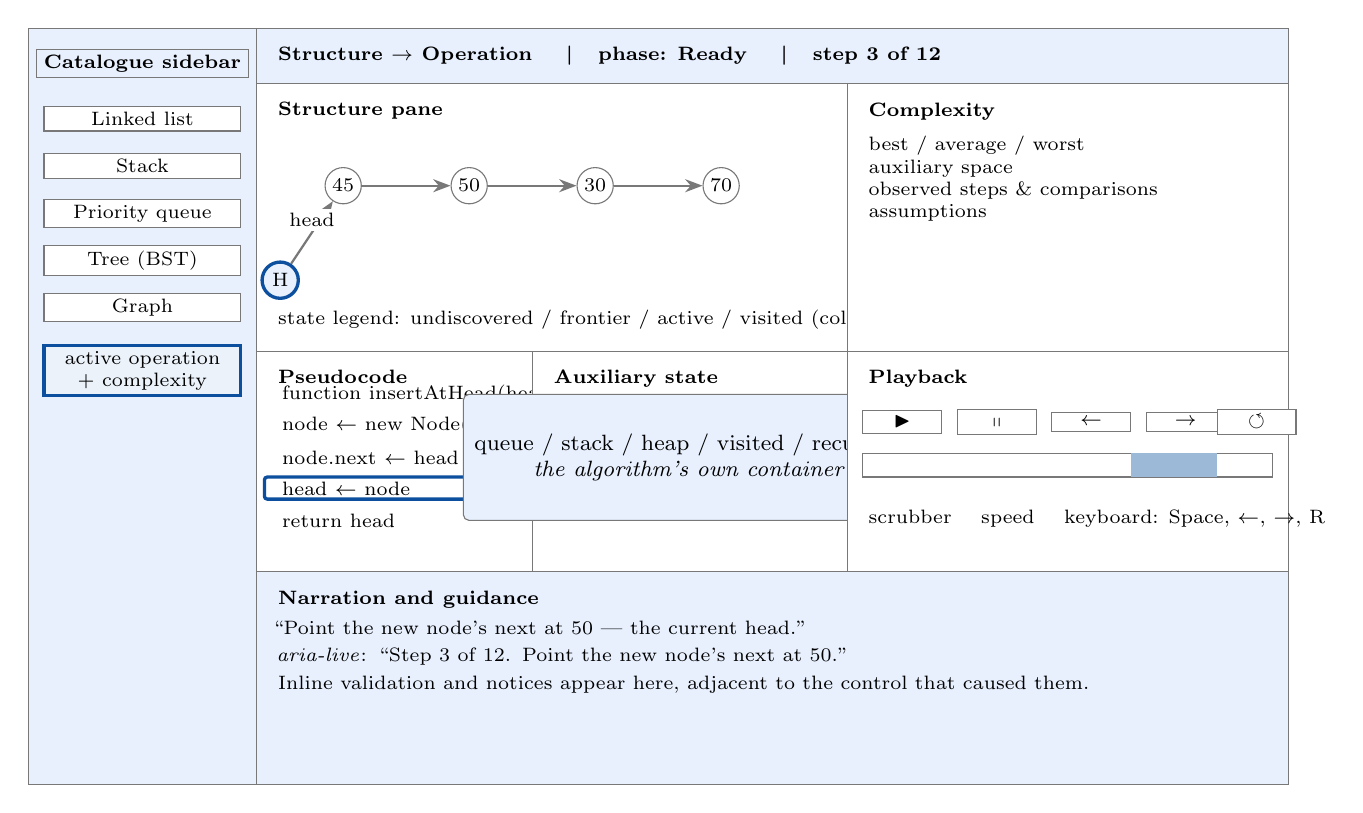
\begin{tikzpicture}[font=\scriptsize, x=1cm, y=1cm]
  % outer shell
  \draw[draw=rulec, fill=codec] (0,0) rectangle (16,9.6);
  % sidebar
  \draw[draw=rulec, fill=statec] (0,0) rectangle (2.9,9.6);
  \node[wfh, minimum width=2.7cm] at (1.45,9.15) {Catalogue sidebar};
  \node[wf, minimum width=2.5cm] at (1.45,8.45) {Linked list};
  \node[wf, minimum width=2.5cm] at (1.45,7.85) {Stack};
  \node[wf, minimum width=2.5cm] at (1.45,7.25) {Priority queue};
  \node[wf, minimum width=2.5cm] at (1.45,6.65) {Tree (BST)};
  \node[wf, minimum width=2.5cm] at (1.45,6.05) {Graph};
  \node[wf, minimum width=2.5cm, fill=boxc, draw=primary, very thick] at (1.45,5.25)
    {active operation\\ + complexity};
  % header
  \draw[draw=rulec, fill=statec] (2.9,8.9) rectangle (16,9.6);
  \node[anchor=west] at (3.05,9.25) {\bfseries Structure $\to$ Operation \quad
    \textbar\quad phase: Ready \quad \textbar\quad step 3 of 12};
  % structure pane
  \draw[wf] (2.9,5.5) rectangle (10.4,8.9);
  \node[anchor=north west] at (3.05,8.78) {\bfseries Structure pane};
  \node[n] (a) at (4.0,7.6) {45};
  \node[n] (b) at (5.6,7.6) {50};
  \node[n] (c) at (7.2,7.6) {30};
  \node[n] (d) at (8.8,7.6) {70};
  \draw[e] (a) -- (b); \draw[e] (b) -- (c); \draw[e] (c) -- (d);
  \node[nactive] (h) at (3.2,6.4) {H};
  \draw[e] (h) -- node[lbl,above]{head} (a);
  \node[anchor=south west] at (3.05,5.65) {state legend: undiscovered / frontier / active /
    visited (colour $+$ label)};
  % pseudocode pane
  \draw[wf] (2.9,2.7) rectangle (6.4,5.5);
  \node[anchor=north west] at (3.05,5.38) {\bfseries Pseudocode};
  \foreach \y/\t in {4.95/{function insertAtHead(head, value):},
                     4.55/{  node $\leftarrow$ new Node(value)},
                     4.15/{  node.next $\leftarrow$ head},
                     3.75/{  head $\leftarrow$ node},
                     3.35/{  return head}} {
    \node[anchor=west] at (3.1,\y) {\t};
  }
  \draw[draw=primary, very thick, rounded corners=1pt] (3.0,3.62) rectangle (6.3,3.9);
  % aux pane
  \draw[wf] (6.4,2.7) rectangle (10.4,5.5);
  \node[anchor=north west] at (6.55,5.38) {\bfseries Auxiliary state};
  \node[auxbox, minimum width=3.6cm, minimum height=1.6cm] at (8.4,4.15)
    {queue / stack / heap / visited / recursion\\ \emph{the algorithm's own container}};
  % complexity column
  \draw[wf] (10.4,5.5) rectangle (16,8.9);
  \node[anchor=north west] at (10.55,8.78) {\bfseries Complexity};
  \node[anchor=north west, align=left] at (10.55,8.35)
    {best / average / worst\\ auxiliary space\\ observed steps \& comparisons\\ assumptions};
  % controls column
  \draw[wf] (10.4,2.7) rectangle (16,5.5);
  \node[anchor=north west] at (10.55,5.38) {\bfseries Playback};
  \node[wf, minimum width=1.0cm] at (11.1,4.6) {$\blacktriangleright$};
  \node[wf, minimum width=1.0cm] at (12.3,4.6) {$\shortparallel$};
  \node[wf, minimum width=1.0cm] at (13.5,4.6) {$\leftarrow$};
  \node[wf, minimum width=1.0cm] at (14.7,4.6) {$\rightarrow$};
  \node[wf, minimum width=1.0cm] at (15.6,4.6) {$\circlearrowleft$};
  \draw[draw=rulec, fill=white] (10.6,3.9) rectangle (15.8,4.2);
  \fill[primary!40] (14.0,3.9) rectangle (15.1,4.2);
  \node[anchor=north west, align=left] at (10.55,3.6) {scrubber \quad speed \quad
    keyboard: Space, $\leftarrow$, $\rightarrow$, R};
  % narration bar
  \draw[draw=rulec, fill=statec] (2.9,0) rectangle (16,2.7);
  \node[anchor=north west] at (3.05,2.58) {\bfseries Narration and guidance};
  \node[anchor=north west, align=left, text width=12.1cm] at (3.05,2.2)
    {``Point the new node's next at 50 --- the current head.''\\[2pt]
     \emph{aria-live}: ``Step 3 of 12. Point the new node's next at 50.''\\[2pt]
     Inline validation and notices appear here, adjacent to the control that caused them.};
  % vertical divider labels
  \node[anchor=west] at (11.6,6.6) {};
\end{tikzpicture}
\caption{Wireframe of the operation workspace (V2). The sidebar and the narration bar persist;
the three panes are always the structure, the pseudocode and the auxiliary state at the same
index; the complexity card and the controls sit beside them. This is a wireframe: it fixes
regions and information, not styling.}
\label{fig:workspace}
\end{figure}

\begin{figure}[htbp]
\centering
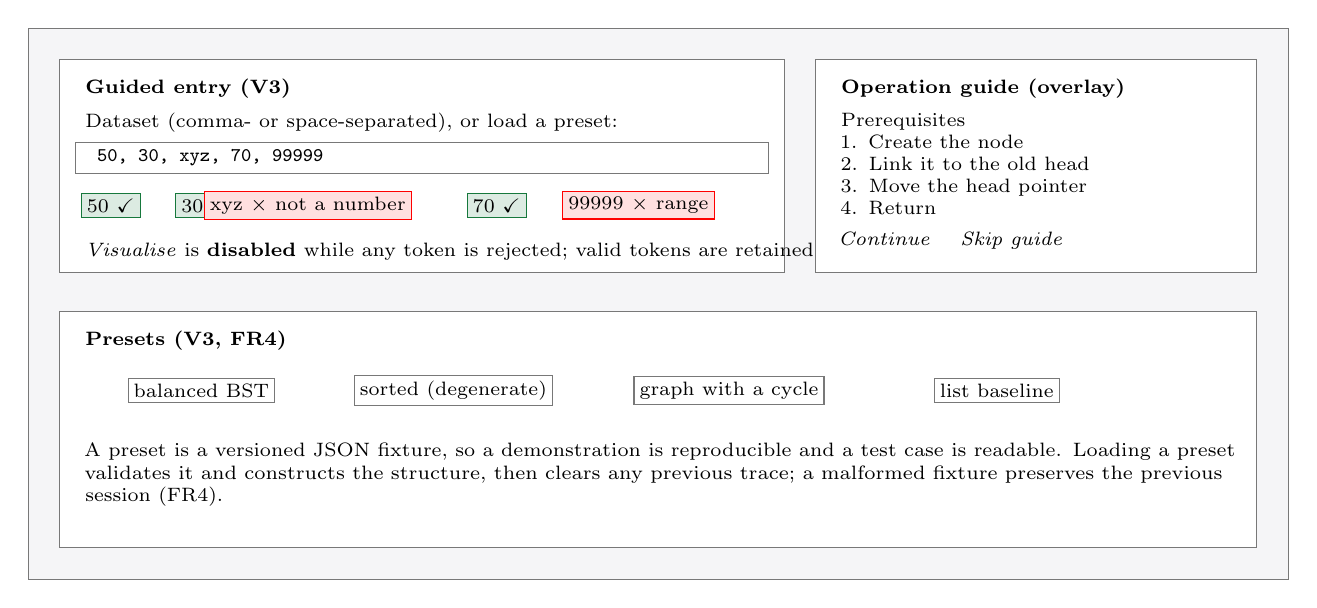
\begin{tikzpicture}[font=\scriptsize, x=1cm, y=1cm]
  \draw[draw=rulec, fill=codec] (0,0) rectangle (16,7.0);
  % entry card
  \draw[wf] (0.4,3.9) rectangle (9.6,6.6);
  \node[anchor=north west] at (0.6,6.48) {\bfseries Guided entry (V3)};
  \node[anchor=north west, align=left] at (0.6,6.05)
    {Dataset (comma- or space-separated), or load a preset:};
  \draw[draw=rulec, fill=white] (0.6,5.15) rectangle (9.4,5.55);
  \node[anchor=west] at (0.75,5.35) {\ct{50, 30, xyz, 70, 99999}};
  % token chips
  \node[wf, fill=okc!15, draw=okc]  at (1.05,4.75) {50 \checkmark};
  \node[wf, fill=okc!15, draw=okc]  at (2.25,4.75) {30 \checkmark};
  \node[wf, fill=red!12, draw=red]  at (3.55,4.75) {xyz $\times$ not a number};
  \node[wf, fill=okc!15, draw=okc]  at (5.95,4.75) {70 \checkmark};
  \node[wf, fill=red!12, draw=red]  at (7.75,4.75) {99999 $\times$ range};
  \node[anchor=north west, align=left] at (0.6,4.4)
    {\emph{Visualise} is \textbf{disabled} while any token is rejected; valid tokens are
     retained, so correcting the two bad ones is enough.};
  % guide overlay
  \draw[wf] (10.0,3.9) rectangle (15.6,6.6);
  \node[anchor=north west] at (10.2,6.48) {\bfseries Operation guide (overlay)};
  \node[anchor=north west, align=left, text width=5.1cm] at (10.2,6.05)
    {Prerequisites\\ 1. Create the node\\ 2. Link it to the old head\\ 3. Move the head
     pointer\\ 4. Return\\[3pt] \emph{Continue} \quad \emph{Skip guide}};
  % preset row
  \draw[wf] (0.4,0.4) rectangle (15.6,3.4);
  \node[anchor=north west] at (0.6,3.28) {\bfseries Presets (V3, FR4)};
  \node[wf] at (2.2,2.4) {balanced BST};
  \node[wf] at (5.4,2.4) {sorted (degenerate)};
  \node[wf] at (8.9,2.4) {graph with a cycle};
  \node[wf] at (12.3,2.4) {list baseline};
  \node[anchor=north west, align=left, text width=14.6cm] at (0.6,1.85)
    {A preset is a versioned JSON fixture, so a demonstration is reproducible and a test case
     is readable. Loading a preset validates it and constructs the structure, then clears any
     previous trace; a malformed fixture preserves the previous session (FR4).};
\end{tikzpicture}
\caption{Wireframe of the guided entry and presets (V3). Validation feedback is per token and
adjacent to the input; the operation guide is an overlay so the workspace is never lost.}
\label{fig:entry}
\end{figure}

\begin{figure}[htbp]
\centering
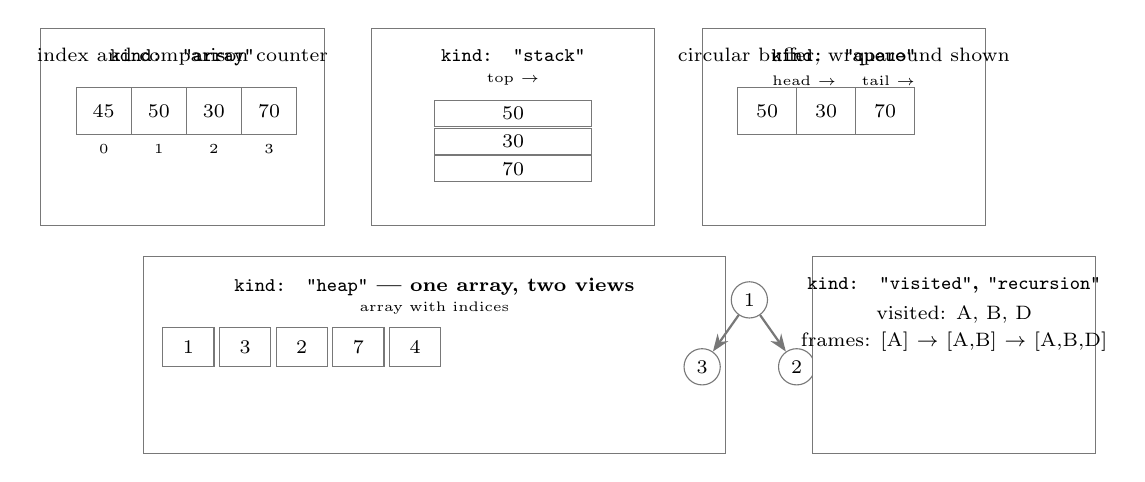
\begin{tikzpicture}[font=\scriptsize, x=1cm, y=1cm]
  % array
  \node[wf, minimum width=3.6cm, minimum height=2.5cm] (arr) at (2.2,4.4) {};
  \node[anchor=north] at (2.2,5.5) {\bfseries \ct{kind: "array"}};
  \foreach \x/\v in {0/45, 1/50, 2/30, 3/70} {
    \draw[draw=rulec, fill=white] (0.85+\x*0.7,4.3) rectangle (1.55+\x*0.7,4.9);
    \node at (1.2+\x*0.7,4.6) {\v};
    \node[font=\tiny] at (1.2+\x*0.7,4.12) {\x};
  }
  \node[anchor=south] at (2.2,5.05) {index and comparison counter};
  % stack
  \node[wf, minimum width=3.6cm, minimum height=2.5cm] (st) at (6.4,4.4) {};
  \node[anchor=north] at (6.4,5.5) {\bfseries \ct{kind: "stack"}};
  \foreach \y/\v in {3.7/70, 4.05/30, 4.4/50} {
    \draw[draw=rulec, fill=white] (5.4,\y) rectangle (7.4,\y+0.33);
    \node at (6.4,\y+0.165) {\v};
  }
  \node[anchor=south, font=\tiny] at (6.4,4.8) {top $\to$};
  % queue circular buffer
  \node[wf, minimum width=3.6cm, minimum height=2.5cm] (q) at (10.6,4.4) {};
  \node[anchor=north] at (10.6,5.5) {\bfseries \ct{kind: "queue"}};
  \foreach \x/\v in {0/50, 1/30, 2/70} {
    \draw[draw=rulec, fill=white] (9.25+\x*0.75,4.3) rectangle (10.0+\x*0.75,4.9);
    \node at (9.625+\x*0.75,4.6) {\v};
  }
  \node[anchor=south, font=\tiny] at (10.6,4.8) {head $\to$ \quad tail $\to$};
  \node[anchor=south] at (10.6,5.05) {circular buffer, wraparound shown};
  % heap
  \node[wf, minimum width=7.4cm, minimum height=2.5cm] (hp) at (5.4,1.5) {};
  \node[anchor=north] at (5.4,2.6) {\bfseries \ct{kind: "heap"} --- one array, two views};
  \foreach \x/\v in {0/1, 1/3, 2/2, 3/7, 4/4} {
    \draw[draw=rulec, fill=white] (1.95+\x*0.72,1.35) rectangle (2.6+\x*0.72,1.85);
    \node at (2.275+\x*0.72,1.6) {\v};
  }
  \node[n] (h0) at (9.4,2.2) {1};
  \node[n] (h1) at (8.8,1.35) {3};
  \node[n] (h2) at (10.0,1.35) {2};
  \draw[e] (h0) -- (h1); \draw[e] (h0) -- (h2);
  \node[anchor=south, font=\tiny] at (5.4,1.9) {array with indices};
  % visited / recursion
  \node[wf, minimum width=3.6cm, minimum height=2.5cm] (vis) at (12.0,1.5) {};
  \node[anchor=north] at (12.0,2.6) {\bfseries \ct{kind: "visited"}, \ct{"recursion"}};
  \node[anchor=north, align=center] at (12.0,2.25)
    {visited: A, B, D\\[2pt] frames: [A] $\to$ [A,B] $\to$ [A,B,D]};
\end{tikzpicture}
\caption{The auxiliary panel is one component per \ct{aux.kind} (FR10). The heap is shown
simultaneously as an array and as a complete binary tree, from one model, so the two views
cannot disagree; the queue shows its circular-buffer head and tail.}
\label{fig:aux}
\end{figure}

\subsection{Controls}

\A\ Table~\ref{tab:controls} is the control inventory. Every control maps to a requirement and
to a controller command; every keyboard binding maps to the same command as the
corresponding button.

{\footnotesize
\setlength{\tabcolsep}{4pt}
\begin{longtable}{@{}L{3.0cm}L{4.0cm}L{3.0cm}L{3.3cm}@{}}
\caption{Control inventory. ``Binding'' names the keyboard key where one exists; the keyboard
and the button invoke the same controller command.}\label{tab:controls}\\
\toprule
\textbf{Control} & \textbf{Action} & \textbf{Feedback} & \textbf{Binding / requirement} \\
\midrule
\endfirsthead
\toprule
\textbf{Control} & \textbf{Action} & \textbf{Feedback} & \textbf{Binding / requirement} \\
\midrule
\endhead
\bottomrule
\endlastfoot
Structure list & Select a structure; open its landing panel & Sidebar highlights the
selection; landing panel updates & Click; FR1 \\
Operation list & Select an operation; open V3 & Operation guide and complexity card load &
Click; FR2, FR3 \\
Preset selector & Load a curated dataset & Structure renders at step~0; preset name shown;
trace cleared & Click; FR4, FR13 \\
Values field & Type or paste values & Per-token chips with reasons; preview of accepted
dataset & Type; FR5, FR6 \\
Target field & Provide a search/delete key & Validated as a single value & Type; FR5 \\
\emph{Visualise} & Validate, build, execute, load & Disabled while input is invalid; success
loads step~0 & Click or Enter; FR7 \\
\emph{Play} / \emph{Pause} & Start / stop the single timer & Phase label; controls enable and
disable; step counter advances & Button or Space; FR11, NFR-U2 \\
\emph{Step back} / \emph{Step forward} & Move the index by $\pm 1$, clamped & Panes update;
narration and live region update; control disabled at the bound & Buttons or
$\leftarrow$ / $\rightarrow$; FR11 \\
\emph{Restart} & Index to $0$, phase to READY & Panes return to step~0; trace not recomputed &
Button or \ct{R}; FR13 \\
Speed & Change the step interval & The new rate applies from the next step & Selector;
FR11 \\
Scrubber & Seek to an arbitrary index & A frame is reconstructed from the nearest checkpoint &
Drag; FR11 \\
Panel collapse & Hide/show a pane & Layout remembers the preference (localStorage) &
Click; FR8--FR10 \\
\end{longtable}
}

\subsection{User workflow}

\R\ The workflow follows UC1 $\to$ UC2 and the five-stage pipeline of Assignment~2 \S5.3, and is
front-loaded so that the animation confirms an expectation rather than substituting for one.

\begin{enumerate}[leftmargin=1.6em,topsep=2pt,itemsep=1pt]
  \item \textbf{Orient and choose} (V1 $\to$ V3): the catalogue opens on a populated workspace
        (a default preset and trace), and selecting an operation opens its guide and complexity
        card before anything runs.
  \item \textbf{Supply data} (V3): keep a preset or type values and an optional target; every
        token is classified immediately and the preview shows exactly what will be used.
  \item \textbf{Visualise} (V3 $\to$ V2): the pipeline runs (parse $\to$ validate $\to$ build
        $\to$ execute $\to$ \ct{controller.load}); the workspace shows step~0 in READY.
  \item \textbf{Explore} (V2): play, pause, step, scrub and restart are all operations on one
        index, with narration, live region and the complexity card tracking each step.
  \item \textbf{Compare and recover} (V2/V3): change the preset or algorithm to compare runs,
        or correct rejected input and re-run --- an illegal operation is a disabled control with
        a reason, never a failure.
\end{enumerate}

\subsection{Feedback for successful operations}

\A\ Feedback is placed next to the thing it describes. \emph{Before execution} the complexity
card states the best/average/worst time and auxiliary space with assumptions in words, and the
guide has said what will happen. \emph{On each step} the narration bar gives one plain-English
sentence, the pseudocode highlights the executing line, the structure highlights the active
node and pointer, the auxiliary panel shows the algorithm's own container with the change since
the previous step emphasised, and the counter reads ``step $i$ of $n$''; the live region
announces the same text (NFR-U2, NFR-U3). \emph{On completion} the last step says what changed
and why it cost what it cost, the card shows observed against theoretical counts, and the final
structure is the confirmable result. Changing a preset or algorithm leaves both runs
inspectable, so a difference is a number and a picture rather than an assertion.

\subsection{Feedback for errors and invalid input}

\R\ ER1--ER13 define the behaviour; Table~\ref{tab:feedback} states where the user sees it. The
principle is that an error is a message about the algorithm, phrased in the user's domain ---
not a stack trace, and not a silent no-op.

\begin{table}[H]
\centering
\small
\setlength{\tabcolsep}{4pt}
\begin{tabular}{@{}L{2.4cm}L{4.0cm}L{3.4cm}L{3.5cm}@{}}
\toprule
\textbf{Situation} & \textbf{What the user sees} & \textbf{Placement} & \textbf{Recovery} \\
\midrule
Non-integer or out-of-range token (ER1, ER2) & The token is marked with its reason; valid
tokens are kept & Inline beside the field, per token & Edit the token; \emph{Visualise}
re-enables automatically \\
Empty or all-invalid dataset (ER3) & Empty-state hint with a valid example; \emph{Visualise}
disabled & Under the field & Provide values \\
Duplicate key (ER4) & The walk is shown; ``equal --- skipped'' notice & Notice region, next to
the workspace & Run continues; the user may remove the duplicate \\
Absent search/delete target (ER5) & The examined path stays highlighted; a ``not present''
banner & Notice region & Run completes; full cost is visible \\
Empty stack / queue (ER6) & Control disabled with a tooltip; keyboard command ignored with an
explicit message & On the control and in the notice region & No state change; run continues \\
Capacity exceeded (ER7) & Refusal names the capacity; capacity badge highlighted; auto-grow
note & On the structure and the notice region & Run continues with existing contents \\
Too many tokens (ER8) & Whole batch refused, with count and limit; nothing partial loaded &
Under the field & Split the input or use a preset \\
Malformed graph (ER9) & Per-line error list; previous graph untouched & Under the edge-list
field, per line & Fix the lines; load is atomic \\
Unreachable vertices (ER10) & ``$k$ of $n$ vertices reachable from \ct{A}''; component muted &
Notice region and structure pane & Restart from another source \\
Trace truncation (ER11) & Banner: trace truncated at the budget; reduce input & Above the
workspace & Reduce input \\
Rapid play/pause (ER12) & No visible error; commands coalesce & --- & Idempotent commands \\
Panel render failure (ER13) & The pane shows a fallback with \emph{Reset visualiser}; other
panes stay usable & In the failing pane & Reset the pane or the session \\
\bottomrule
\end{tabular}
\caption{Error feedback: what the user sees, where it appears, and how the session recovers.
This is the interface form of the ER table of Assignment~1 \S3.3.}
\label{tab:feedback}
\end{table}

\noindent\textbf{Principles.} \A\ (i)~Errors are never modal for invalid \emph{data}: the user
keeps editing. (ii)~A message names the offending value and the reason, never ``invalid
input''. (iii)~Disabled is preferred to failing: if a control cannot succeed, it is disabled
with a reason. (iv)~Errors do not destroy context: a malformed graph or preset leaves the
previous session intact. (v)~Errors are announced to assistive technology as well as drawn.

\subsection{Responsiveness and layout}

\R\ NFR-Po2 fixes the layout: the workspace collapses to a stacked layout below 1024~px, the
sidebar to icons below 768~px, and the design target is a classroom projector at
$1280\times720$. \A\ The layout is desktop-first for that target, with a graceful narrow mode:
the full three-pane workspace of Figure~\ref{fig:workspace} above 1280~px; the complexity card
and controls below the panes at 1024--1280~px with no horizontal scroll; a stacked workspace
with a pinned narration bar at 768--1024~px; an icon sidebar with tabbed panes below 768~px (a
courtesy mode, not the target); a pan-and-zoom viewport with an explicit cap note above the
caps (NFR-S1); and internally scrolling narration and pseudocode, with the executing line
auto-scrolled into view (FR9), while the structure pane pans and zooms without reflowing the
algorithm's state.

\subsection{Accessibility and usability}

\R\ The target is WCAG~2.1 AA (NFR-U2). \A\ \emph{Keyboard}: every control is reachable and
operable, focus order follows visual order, and the keyboard path invokes the same controller
commands as the buttons. \emph{Announcements}: step changes update an ARIA live region, and
validation rejects and error notices are announced; the counter has a text label.
\emph{Perceivable state}: contrast at least 4.5:1 and node state carried by colour \emph{and} a
label or shape. \emph{Motion}: \ct{prefers-reduced-motion} replaces interpolation with
instantaneous steps, affecting only the view. \emph{Structure}: semantic landmarks and headings,
a focus-trapping guide overlay, and a focusable error-boundary fallback. \emph{Usability}:
NFR-U1 targets the UC1 $\to$ UC2 flow in under three minutes at 80\% success across five users;
a populated first paint, an in-context guide, presets and per-step narration support it, and
the five-user check runs in Phase~5.

%=======================================================================
\section{Risks, Assumptions, and Limitations}

The brief asks for at least three technical risks with a mitigation each, at least three
assumptions, and at least three anticipated limitations. We give eight, seven and eight
respectively, because the honest risks of this project are not all technical and not all
alike.

\subsection{Technical risks and mitigations}

{\footnotesize
\setlength{\tabcolsep}{4pt}
\begin{longtable}{@{}L{0.8cm}L{3.5cm}L{1.3cm}L{1.3cm}L{6.6cm}@{}}
\caption{Technical and delivery risks, with impact, likelihood and the mechanism that enforces
each mitigation.}\label{tab:risks}\\
\toprule
\textbf{ID} & \textbf{Risk} & \textbf{Impact} & \textbf{Likelihood} & \textbf{Mitigation and enforcement} \\
\midrule
\endfirsthead
\toprule
\textbf{ID} & \textbf{Risk} & \textbf{Impact} & \textbf{Likelihood} & \textbf{Mitigation and enforcement} \\
\midrule
\endhead
\bottomrule
\endlastfoot
R1 & \textbf{Scope:} five structures and their operations are a large surface for two people,
so the graded set is not finished by the deadline & High & Medium & Build one vertical slice
first (done), freeze the \ct{Step} contract (ADR-8), then add operations additively; each
operation is one generator \(+\)
one listing \(+\)
one catalogue record (NFR-S2). Phase gates in Section~7 make the remaining surface visible
weekly, and the contract freeze means a slip delays a feature, not the architecture \\
R2 & \textbf{Two rendering paradigms:} mixing D3's DOM mutation with React's rendering
produces stale elements or flicker, especially on step-back & High & Medium & ADR-2 is
absolute for the main visualisation: D3 computes geometry, React owns the SVG; \ct{d3-selection}
is not used for the main view; the step-back DOM-equality test of T12 fails if a stale element
survives \\
R3 & \textbf{Non-determinism:} an unseeded random layout or neighbour order makes traces
irreproducible, breaking golden tests and exact replay & High & Medium & No wall-clock and no
randomness in the core (ADR-8 D7); the neighbour order is fixed to adjacency insertion order
and displayed; \ct{d3-force} is relaxed once with a fixed seed and frozen; an ESLint rule bans
\ct{Math.random} in \ct{core/}; golden traces catch any drift (NFR-C2) \\
R4 & \textbf{Performance at the cap:} aggregate generation or SVG reconciliation exceeds the
frame or latency budget at $n = 200$ & Medium & Medium & Precompute the trace and replay it;
run large generation in a Web Worker; keep per-frame state $O(n)$ with stable keys and
memoised panes; freeze the force layout; measure the budgets in CI (\S3.6) and degrade to
pan-and-zoom or truncate with disclosure (ER11) \\
R5 & \textbf{Content drift:} the pseudocode listing, the \ct{codeLine} map and the complexity
card disagree with the generator after a change & Medium & Medium & One \ct{OperationMeta}
record is the single source for the label, the listing id and the bounds; a completeness test
asserts every operation has a listing and a full line map; the golden trace changes in the same
pull request (FR3, FR9) \\
R6 & \textbf{Per-structure bugs in the model:} an invariant (heap property, BST ordering,
acyclicity) silently breaks and the animation teaches something wrong & High & Medium &
Invariants are asserted at every step of every trace, not only at the end (NFR-C4); every
operation is checked against an independent reference and the C textbook functions (NFR-C1);
property tests cover randomised inputs \\
R7 & \textbf{Test rot in the UI:} interaction tests written against the visual design break on
every restyle, so the team starts skipping them & Medium & Medium & Locate by role, accessible
name and text, never by class or pixel; golden \emph{traces} are the stable regression
artefact; screenshot tests are deliberately not used; one E2E walkthrough, not many \\
R8 & \textbf{Browser/worker compatibility:} \ct{structuredClone}, Web Worker or modern
ES features are unavailable in an older browser used by a grader & Low & Low & Target the last
two versions of the major browsers (NFR-Po1); feature-detect the worker and fall back to
main-thread generation; the app remains a static bundle with no server dependency \\
\end{longtable}
}

\subsection{Assumptions}

\begin{itemize}[leftmargin=1.4em,topsep=2pt,itemsep=1pt]
  \item \textbf{A1. Graded scope.} \A\ Linked list, stack, priority queue, tree (BST) and graph
        are graded; the FIFO queue is supporting and the traversals plus BFS/DFS are the graded
        algorithms (Assignment~2 \S2.1, ADR-5). A promotion is additive.
  \item \textbf{A2. Small inputs by design.} \A\ Teaching-sized data ($\le 100$ linear,
        $\le 200$ tree/graph); large-scale streaming is out of scope (NFR-S1).
  \item \textbf{A3. A modern evergreen browser on a conventional machine.} \A\ A 2020-era
        laptop with 8~GB of RAM on the latest stable Chrome; the budgets of \S4 assume it.
  \item \textbf{A4. Standard, unweighted algorithms.} \A\ Unweighted BFS and DFS; weighted
        shortest paths, self-balancing trees and union--find are out of scope (Assignment~2
        \S3.8).
  \item \textbf{A5. Data, not code.} \A\ Input is values and an edge list, never executable
        content; no \ct{eval} and no server, so no injection or data-at-rest surface
        (NFR-Se1).
  \item \textbf{A6. Determinism is achievable and desirable.} \A\ A fixed neighbour order and a
        seeded or frozen layout make every trace byte-identical, which is what golden tests and
        exact replay require (NFR-C2).
  \item \textbf{A7. Two people work in parallel against one frozen interface.} \A\ The
        \ct{Step} contract (ADR-8) and the layer boundaries (NFR-M2) are the coordination
        mechanism; both members review before merge.
\end{itemize}

\subsection{Anticipated limitations}

\begin{itemize}[leftmargin=1.4em,topsep=2pt,itemsep=1pt]
  \item \textbf{L1. A teaching visualiser, not an algorithm library.} \A\ It visualises its own
        operations step by step; it does not accept arbitrary user code.
  \item \textbf{L2. No persistence, sharing or accounts.} \A\ Without a backend (NFR-Se1) a
        session is not saved or resumed; traces export only as a fixture file.
  \item \textbf{L3. Legibility and animation degrade above the caps.} \A\ Beyond the caps the
        SVG pan-and-zoom is a workaround; the interface states the cap rather than degrading
        silently (NFR-S1).
  \item \textbf{L4. ``Observed step count'' is a model charge.} \A\ It counts emitted events and
        comparisons, not CPU cycles, and the complexity card says so.
  \item \textbf{L5. Accessibility is self-audited to WCAG~2.1 AA, not certified.} \A\ A formal
        audit and an exhaustive screen-reader matrix are outside the assignment's scope.
  \item \textbf{L6. Mobile and touch are courtesy modes.} \A\ The target is a
        $1280 \times 720$ projector and a desktop pointer; narrow layouts stack but a
        first-class touch experience is not a goal.
  \item \textbf{L7. The C reference functions are reading aids and test oracles.} \A\ They are
        the textbook algorithms (Assignment~2 \S3), not the shipped implementation.
  \item \textbf{L8. The visualised algorithm set is fixed for this iteration.} \A\ Dijkstra,
        $A^{*}$, topological sort, SCC and self-balancing trees are excluded (Assignment~2
        \S3.8); some are additive later, none is promised now.
\end{itemize}

%=======================================================================
\section{Development Plan}

The brief lists six phases and asks for a short plan with responsibilities and expected
outcomes, and for a description of how Git/GitHub will be used for regular, meaningful
commits and collaborative development.

\subsection{Phases, responsibilities and outcomes}

\R\ Table~\ref{tab:phases} follows the brief's six phases and adds an exit criterion and a
status for each. \A\ Responsibility is split by layer, because that is where the frozen
interface already divides the work: one member owns the core domain (models, generators,
trace store, oracles), the other owns the application and presentation layers (validation
plumbing, controller, worker, renderers, panes, accessibility), and both own the contract and
integration. Splitting by layer rather than by structure is deliberate: it keeps one person's
edits from spanning the boundary that the other person is responsible for.

\begin{table}[H]
\centering
\small
\setlength{\tabcolsep}{4pt}
\begin{tabular}{@{}L{0.7cm}L{4.3cm}L{2.6cm}L{3.2cm}L{3.0cm}@{}}
\toprule
\textbf{\#} & \textbf{Work} & \textbf{Responsible} & \textbf{Expected outcome} &
\textbf{Exit criterion / status} \\
\midrule
1 & Review requirements and technical design; confirm scope and the frozen contract &
Both (joint) & Agreed scope, ADRs, and the trace contract at v1 &
\done\ ADR-8 accepted; A1/A2 frozen \\
2 & Core data structures and system layer: five models, trace store, validator, controller,
state machine, worker & P.\ Morindat (models, store); Y.\ Megenta (controller, state machine,
validator, worker) & Every structure and system component present and unit-tested, with the
list slice fully working &
Partial: list model, store, controller, state machine and validator done (25 core tests pass);
the other four models are typed stubs \\
3 & Algorithms and core functionality: list/stack/heap/BST operations, the four traversals,
BFS and DFS, with instrumentation and complexity metadata & P.\ Morindat (generators); Y.\
Megenta (catalogue content, pseudocode listings, line maps) & Every graded operation emits a
correct, deterministic \ct{Step[]} and has a golden trace &
Not started; the \ct{insertAtHead} generator is the template and the contract is frozen \\
4 & UI/UX integration: structure renderers and layout, the three panes, controls, guide,
validation feedback, accessibility & Y.\ Megenta (renderers, panes, controls, a11y); P.\
Morindat (layout geometry, worker client) & The workspace of Figure~\ref{fig:workspace}
driven entirely by \ct{(trace, index)} &
Partial: shell, panes and list renderer exist for the slice; the other renderers and the full
control set are scheduled \\
5 & Testing and debugging: property and differential tests, integration, UI tests, golden
traces, performance budgets & Both, cross-reviewing & The suite of Section~3 green in CI, with
coverage at or above 90\% on \ct{src/core/**} &
Not started beyond the slice's 25 tests \\
6 & Final refinement and documentation: accessibility pass, usability check, README and ADR
updates, the demo script and the recorded walkthrough & Both (joint) & A demonstrable,
documented submission & Not started \\
\bottomrule
\end{tabular}
\caption{The six-phase development plan. ``Partial'' means the vertical slice satisfies part of
the phase; the status column is deliberately falsifiable against the repository.}
\label{tab:phases}
\end{table}

\subsection{Schedule and sequencing}

\A\ The plan is risk-first: the contract and the hardest integration points are settled early,
and the content that scales with the structure count is added last, when the pattern is
proven. Figure~\ref{fig:timeline} shows the six phases over six working weeks, with the
hardening phases overlapping the feature phases on purpose so that tests are written with
each feature rather than after all of them.

\begin{figure}[htbp]
\centering
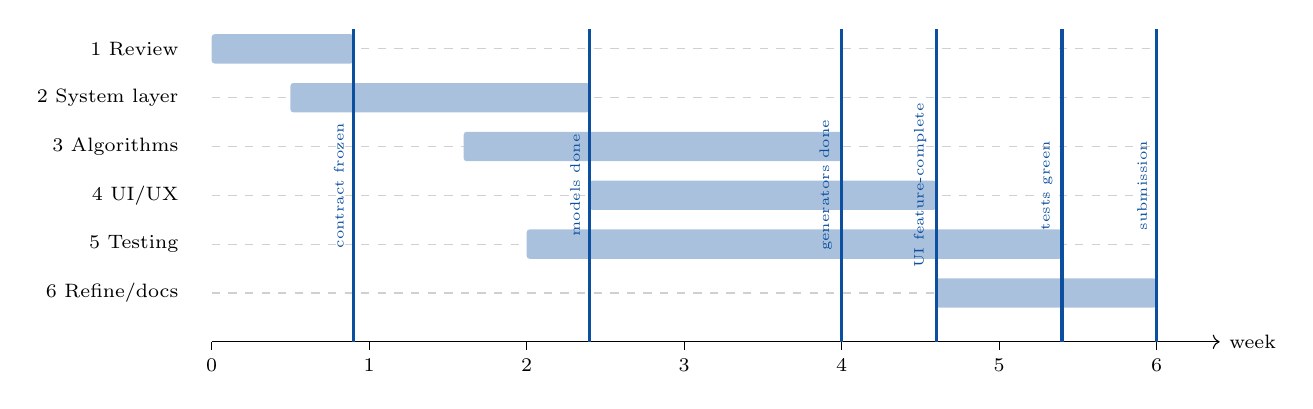
\begin{tikzpicture}[font=\scriptsize, x=2.0cm, y=0.62cm]
  % axes / weeks
  \draw[->] (0,0) -- (6.4,0) node[right]{week};
  \foreach \w in {0,1,2,3,4,5,6} {
    \draw (\w,0) -- (\w,-0.16);
    \node[below] at (\w,-0.16) {\w};
  }
  \foreach \y in {1,...,6} {
    \draw[rulec!35, dashed] (0,\y) -- (6,\y);
  }
  % labels
  \node[anchor=east] at (-0.15,6) {1 Review};
  \node[anchor=east] at (-0.15,5) {2 System layer};
  \node[anchor=east] at (-0.15,4) {3 Algorithms};
  \node[anchor=east] at (-0.15,3) {4 UI/UX};
  \node[anchor=east] at (-0.15,2) {5 Testing};
  \node[anchor=east] at (-0.15,1) {6 Refine/docs};
  % bars
  \fill[primary!35, rounded corners=1pt] (0.0,5.7) rectangle (0.9,6.3);
  \fill[primary!35, rounded corners=1pt] (0.5,4.7) rectangle (2.4,5.3);
  \fill[primary!35, rounded corners=1pt] (1.6,3.7) rectangle (4.0,4.3);
  \fill[primary!35, rounded corners=1pt] (2.4,2.7) rectangle (4.6,3.3);
  \fill[primary!35, rounded corners=1pt] (2.0,1.7) rectangle (5.4,2.3);
  \fill[primary!35, rounded corners=1pt] (4.6,0.7) rectangle (6.0,1.3);
  % milestones
  \foreach \x/\lab in {0.9/contract frozen, 2.4/models done, 4.0/generators done,
                       4.6/UI feature-complete, 5.4/tests green, 6.0/submission} {
    \draw[primary, very thick] (\x,0) -- (\x,6.4);
    \node[rotate=90, anchor=south, font=\tiny, text=primary] at (\x,3.2)
      {\lab};
  }
\end{tikzpicture}
\caption{Indicative schedule. Bars are the six phases; vertical lines are the gates that the
plan is actually managed against (the contract freeze is already met, so the plan starts
ahead on Phase~1).}
\label{fig:timeline}
\end{figure}

\subsection{Git and GitHub collaboration}

\R\ Instruction~5 makes the GitHub Classroom repository the submission channel; NFR-M1 and
NFR-M2 make quality enforcement part of the build. \A\ We use a trunk-based workflow with
short-lived branches and mandatory review, because it fits two people and keeps the frozen
contract under review.

\begin{itemize}[leftmargin=1.4em,topsep=2pt,itemsep=1pt,before=\raggedright]
  \item \textbf{\ct{main} is protected}: direct pushes are disabled, and a change lands only
        through a pull request with the other member's approval and all checks green.
  \item \textbf{Short-lived, single-purpose branches} (\ct{feat/bst-insert},
        \ct{test/heap-property}, \ct{docs/a3}, \ct{fix/checkpoint-replay}), merged or closed
        within a phase and deleted after merge.
  \item \textbf{Conventional, meaningful commits}, one logical change each, stating \emph{what}
        and \emph{why}: \ct{feat(bst): insert generator}, \ct{test(heap): heap invariant},
        \ct{docs(a3): testing plan}, \ct{refactor(trace): checkpoint search}.
  \item \textbf{A pull-request checklist}: does this change the \ct{Step} contract (if so, an
        ADR and regenerated golden traces)? does a new operation bring a generator, a listing
        and an \ct{OperationMeta}? are tests, coverage and docs green?
  \item \textbf{Contract changes are a deliberate, visible event} under the ADR-8 policy:
        additive changes bump the version note and regenerate the goldens; breaking changes
        update every producer and consumer and carry a migration note, in one commit;
        \ct{step.test.ts} locks the key set, so even an additive change needs approval. Golden
        traces are committed JSON and reviewed as diffs; \ct{--update} is never run blindly.
  \item \textbf{Issues, milestones and CI mirror the plan}: one issue per operation (acceptance
        criteria as in \S7.4), milestones are the six phases, labels distinguish
        \ct{area:core}, \ct{area:ui}, \ct{type:test}, \ct{type:docs} and \ct{risk}, and GitHub
        Actions runs \ct{typecheck}, \ct{lint}, \ct{test:core} and \ct{build} on every push
        (Phase~5 adds coverage, the payload budget and the E2E walkthrough).
  \item \textbf{Tagged checkpoints and docs with the code}: \ct{v0.1-slice},
        \ct{a3-submission} and phase tags make a demonstration reproducible; the README, the
        ADRs and the \LaTeX{} sources are version-controlled and updated in the same pull
        request as a behaviour change.
\end{itemize}

\subsection{Definition of done for an operation}

\A\ An operation is complete --- and therefore mergeable --- only when all of the following
hold. This is the same list as the PR checklist, in the form the team uses:

\begin{enumerate}[leftmargin=1.6em,topsep=2pt,itemsep=1pt]
  \item an instrumented generator in \ct{core/operations/} that emits a deterministic
        \ct{Step[]} and a \ct{GenerateSummary};
  \item an authored pseudocode listing and a total \ct{codeLine} map, plus its
        \ct{OperationMeta} record with best/average/worst/space and assumptions;
  \item unit tests for the step sequence, deltas and narration; an invariant assertion at
        every step; a reference/oracle test; and a golden-trace fixture;
  \item any new \ct{aux.kind} or renderer needed to display it;
  \item a documentation note if the complexity or the interface changed; and
  \item green CI on the pull request, with the other member's approval.
\end{enumerate}

%=======================================================================
\section{Expected Deliverables}

The brief asks what the final project will ultimately contain. Table~\ref{tab:deliverables}
lists the deliverables, the artefact a grader can inspect for each, and the phase that
produces it. The minimum list of the brief is covered, and four items are added that this
project specifically needs.

\begin{table}[H]
\centering
\small
\setlength{\tabcolsep}{4pt}
\begin{tabular}{@{}L{3.6cm}L{6.6cm}L{4.2cm}@{}}
\toprule
\textbf{Deliverable} & \textbf{What it is} & \textbf{Where / phase} \\
\midrule
Complete source code & Five structure models, the trace contract and store, the instrumented
generators for every graded operation, the traversals, BFS and DFS, the controller and
worker, the renderers and the UI, in the layered repository of Assignment~2 \S5.3 &
\ct{src/}; phases 2--4 \\
System and design documentation & The A1, A2 and A3 documents, the ADR set (including
ADR-8), and an up-to-date README with architecture and trace-contract sections &
\ct{ProjectResources/}, \ct{README.md}; all phases \\
Data representations & The \ct{Step}/\ct{StructureDelta}/\ct{AuxState} contract and the five
model representations, each with its invariants and its cost model & \ct{src/core/},
A2 \S4, A3 \S3--\S4 \\
Algorithm documentation & Per-operation pseudocode listings, the \ct{codeLine} maps, the C
reference functions, and the correctness intuitions of Assignment~2 \S3 &
\ct{src/data/catalogue.ts}, A2 \S3, A3 \S3.4 \\
Complexity analysis & The per-operation bound and auxiliary space, the trace-size and storage
bounds, and the observed-count comparison shown in the interface & A2 \S3--\S4, A3 \S4,
the complexity card \\
Demonstration of the major features & A live demonstration and a recorded walkthrough of the
UC1 $\to$ UC2 flow, a degenerate-versus-balanced BST comparison, a BFS/DFS comparison and a
heap build-versus-inserts comparison & Demo script and recording; phase 6 \\
Representative sample inputs & The versioned presets (balanced BST, sorted/degenerate BST,
graph with a cycle, list baseline) and the golden traces & \ct{src/data/presets/},
\ct{src/data/golden/}; phases 2--5 \\
Associated design assignments & This document and its two predecessors, compiled to PDF under
the required naming conventions & \ct{ProjectResources/}; continuous \\
\emph{Added:} test suite and quality evidence & The DOM-free core suite, property and oracle
tests, UI tests, one E2E walkthrough, golden traces, and the CI configuration that enforces
coverage and the import boundary & \ct{src/**/*.test.ts}, \ct{tests/}, \ct{.github/workflows/};
phases 4--5 \\
\emph{Added:} performance evidence & The budget harness results (generation latency, frame
time, payload, memory) against the \S4 targets & \ct{perf/} and CI; phase 5 \\
\emph{Added:} accessibility statement & A short statement of the WCAG~2.1 AA commitments, what
was tested, and the known limitations (L5) & \ct{README.md} and A3 \S5.8; phases 4--6 \\
\emph{Added:} a demo script & A reproducible path through the tool that exercises the graded
features in a fixed order, so a demonstration is not improvised & \ct{docs/demo.md}; phase 6 \\
\bottomrule
\end{tabular}
\caption{Expected final deliverables, the inspectable artefact, and the phase that produces
each.}
\label{tab:deliverables}
\end{table}

%=======================================================================
\section{Questions for Design Review}

\noindent The eight questions are answered concisely but technically.

\paragraph{1. What is the single most important algorithmic challenge in your project?}
\A\ Instrumenting the algorithms so the trace is \emph{complete and faithful} without changing
the cost model. For the graph searches this is sharpest: BFS and DFS are defined only up to the
order in which neighbours are expanded, so ``the correct trace'' does not exist until that order
is fixed, and a trace that omits the frontier at a dequeue hides exactly the state the learner
needs. We emit one step per meaningful event (dequeue/pop, examine-edge, discover, visit), carry
the algorithm's \emph{own} container in the step's \ct{aux} payload, and fix neighbours to
adjacency insertion order (Assignment~2 \S3.7). The challenge is then to show instrumentation adds
only $O(1)$ per step and that the instrumented result equals the textbook result --- which the C
reference oracle and the metamorphic tests of \S3.4 establish.

\paragraph{2. What is the most appropriate data structure for the central problem, and why?}
\A\ The central problem is not one of the five structures but making an execution addressable by
index, so the answer is the \textbf{immutable \ct{Step} plus a delta log with periodic
checkpoints}. \ct{Step} is snapshot-shaped for its readers, so the interface is a pure function
of \ct{(trace, index)}; the storage is a delta log, so memory is $O(s + (s/k)n)$ rather than
$O(ns)$ and display is independent of the index (ADR-1, ADR-3). The five models match their
textbook representations because that keeps the cost model honest, but the trace is what makes
the tool a visualiser rather than a library with a picture attached.

\paragraph{3. What is the most computationally expensive operation?}
\A\ Two, for different reasons. \emph{Trace generation for an aggregate session}: $n$ sorted BST
insertions produce $\Theta(n^2)$ steps on a degenerate tree ($\Theta(n\log n)$ balanced), each
also applied to the structure to keep generator and store in agreement. \emph{Per-frame rendering
at the cap}: at $n=200$ React reconciles $O(n)$ SVG elements which the browser lays out and
paints. Generation is offloaded to a Web Worker above the threshold, bounded by the step budget
and done once per run; rendering is bounded because no algorithm runs per frame, identifiers are
stable so React reuses DOM, and the force layout is relaxed once and frozen.

\paragraph{4. What happens when the user provides invalid input?}
\A\ Validation is total and precedes construction (ADR-7, FR6): every token is classified
independently and shown with a specific reason, valid tokens are retained, and \emph{Visualise}
is disabled while any token is invalid --- so no trace is generated and the engine is never
reached by raw text (asserted with a spy in \S3.3). Structure-specific rules apply on top:
duplicates are rejected on insert while the comparison walk is still shown (ER4); a graph load is
atomic and reports per-line errors (ER9); and a pop on an empty stack is a disabled control with
a reason, not an exception (ER6).

\paragraph{5. Which component is most likely to change during future development?}
\A\ The \emph{content and catalogue layer} --- pseudocode listings, \ct{codeLine} maps, guide
text and complexity records --- together with the set of \ct{aux} panel kinds and renderers. It
is the layer that grows with scope and the one a course would extend. The \ct{Step} contract was
frozen at v1 (ADR-8) precisely so that it is \emph{not} the churning component; it may grow
additively, but only as a deliberate, ADR-backed event.

\paragraph{6. How does your architecture isolate that component?}
\A\ Content is data, not code: one \ct{OperationMeta} and one pseudocode listing per operation,
read only through \ct{app/catalogue.ts}, so the UI holds no hard-coded bound or listing. Adding
an operation is exactly three edits --- one generator, one listing plus line map, one catalogue
record (Assignment~2 \S5.7, NFR-S2) --- and the controller, state machine and shell stay
untouched. The same isolation bounds \ct{aux} and renderer changes: the \ct{AuxKind} and
\ct{EdgeKind} unions are closed, one panel handles one kind, and a new structure needs one model
and one renderer. The import-boundary lint rule (NFR-M2) enforces the direction.

\paragraph{7. What is one design decision you considered but rejected? Why?}
\A\ \textbf{Recomputing the algorithm's state on demand instead of storing a trace.} It is
simpler to write, costs no storage and is correct for forward stepping, but every move ---
including step-back, which a learner relies on --- would cost $O(i)$, and state that depends on
the run so far (the exact BFS frontier, the recursion depth) could not be represented without
replaying that history. It makes the state \emph{recomputable} rather than \emph{addressable}, so
the UI could not scrub and a timing difference could change what the learner sees. A stored
deterministic trace costs one generation pass and $O(s)$ memory and makes step-back, scrub and
exact replay architectural (ADR-1). A second rejection, in one line: letting \ct{d3-selection}
own the main SVG is a known source of stale elements on step-back (ADR-2).

\paragraph{8. What additional feature could be implemented without redesigning the core
architecture?}
\A\ Several, which is the evidence that the design is extensible. \textbf{Topological sort,
cycle detection and SCC} reuse the DFS generator and add an edge-classification or post-order
rule (one generator, one listing). \textbf{Dijkstra} uses the already-graded priority queue as
its frontier and adds relaxation events. \textbf{Promoting the FIFO queue} to a catalogue entry
is one catalogue record, one generator set and one renderer, since its circular buffer and
\ct{aux.kind} already exist. \textbf{Expression-tree evaluation} is postorder plus an arithmetic
rule, and \textbf{exporting or deep-linking a trace} needs no engine change because the trace is
already serialisable. In every case the \ct{Step} contract, store, controller and shell are
unchanged.

%=======================================================================

\end{document}

